% !TEX root = main.tex

% ==============Chapter 5: Implementation and Deployment===================== %
\chapter{Implementation and Deployment of \Ghazalstar}
\label{chap:Implementation and Deployment}
% ==============Introductory remarks===================== %
\section{Introductory Remarks}

In the previous chapter, we described \Ghazalstar, a new paradigm for a DNS system and certification model which allows entities to securely register domain names and obtain certificates for those names. We also discussed the various design decisions that have been taken into account while designing \Ghazalstar scheme. While Bitcoin scripting language is highly restrictive, the Ethereum blockchain is developed to enable developers to leverage the underlying blockchain security and execute their own programs, known as smart contracts, in a fully decentralized manner. In this chapter, we further detail the implementation and deployment of our system, that is mainly a smart contract written in Solidity, in addition to identifying the security requirements of its functions.

% ==============Ethereum Concepts===================== %
\section{Ethereum Concepts}

What follows is a description of the Ethereum blockchian concepts which draw upon insights into how this technology works and what are the chief components of it.

% ==============Ethereum Accounts===================== %
\subsection{Ethereum Accounts}

Accounts are entities that play the most significant role in the Ethereum blockchain. There are two types of (i) externally owned accounts and (ii) contract accounts on the Ethereum. Both types of Ethereum accounts are associated with a 40-character hexadecimal format public key known as Ethereum address. These accounts, as Ethereum network entities, hold states. Externally owned accounts, referred to accounts, own balance while contract accounts hold balance and contract storage. 
Ethereum nodes keep track of the network's state which is the most recent state of each existing account and is updated with every block that is added to the blockchian. 
% ==============Smart Contracts and Transactions===================== %
\subsection{Smart Contracts and Transactions}
\label{sec:solidity}
As mentioned, a contract is an Ethereum account that contains a piece of code and can be executed on the Ethereum Virtual Machine (EVM). Once deployed on the Ethereum, smart contracts are not executed unless they are called up and triggered by mechanisms known as transactions. Transactions can be originated from either another contracts or normal accounts, in both cases the contract code is executed on the EVM and its state changes based on the transactions it has received as an input. 

Originally, Smart contracts were written and developed high level languages including Mutan (C-like language)~\cite{Mutan·et50:online}, LLL (LISP-like language)~\cite{LLLPoC6·23:online}, and Serpent (Python-like language)~\cite{Serpent·19:online}. However, smart contracts are currently written in Solidity, a high level object oriented language which is similar to Java~\cite{Solidity87:online}.
% ==============Ether===================== %
\subsection{Ether}

Similar to bitcoin, ether (ETH) is a class of cryptocurrency, while it alternatively supplies "fuel" for the Ethereum network to run the decentralized applications. In order for the Ethereum nodes to process and execute a transaction, a transaction fee is required to be paid in ether. These fees are calculated based on the computational resources and the time that is required to execute them, so ether is also called the "digital oil". Like Bitcoin, one can obtain ether by (i) being a miner and verifying network transactions, where every 12 seconds 5 ethers are rewarded to the miner, or (ii) by purchasing from another Ethereum entity.
% ==============Gas===================== %
\subsection{Gas}

As it was mentioned in the above, Ethereum nodes are required to be rewarded for executing the transactions and maintaining the Ethereum blockchain, this is achieved by paying ether for each transaction. The amount of ether in these transaction fees indicate the notion of gas. Every transaction contains a number of operations and there is a precise amount of gas unit associated with each operation. Accordingly, the ultimate amount of gas required for a transaction to be executed is equal to the gas needed for all the operations in that transaction. Each transaction has a corresponding gas price which incentivizes the network nodes to execute it and transactions with higher amount of gas are effectively processed faster by the network. 

It is almost impossible for a sender to examine the precise amount of gas needed for the completed execution of the transaction he aims to send to the network, thus there is a gas limit associated with each transaction. Gas limit is the maximum amount of gas that a sender can pay as a transaction fee so that he does not loose all of his funds. By doing so, the transaction is certainly executed by the network nodes and the remaining gas (if there is any) is refunded to the payee. 
% ==============Mining===================== %
\subsection{Mining}

Like all other blockchain technologies, Ethereum employs a mining process to ensure a secure and valid decentralized record keeping. To do so, a block is broadcast to the network after it is mined by a miner, then it is checked as valid and appended to the blockchain, if it contains a proof of work of a determined difficulty. The proof of work algorithm that is currently applied by the Ethereum is called \emph{Ethash}~\cite{Ethash·e70:online} and it involves finding a nonce input to the algorithm so that the result is below a certain threshold depending on the difficulty. Note that to maintain 12 second block interval in the Ethereum, the mining difficulty fluctuates. 

Miners require to invest high computational resources to perform the proof of work as it contains extremely expensive computations. As a reward, they gain 5 ether for every block they create and mine in addition to total gas consumed by the entire transactions within that block. By doing so, Ethereum provides an incentive for the network nodes (miners) to verify the transactions and maintain a decentralized and immutable ledger of information.

% ==============Design and Implementation===================== %
\section{Design and Implementation}

While the previous section focused on theoretical concepts of the Ethereum blckchain, in this section, we will outline how \Ghazalstar system has been developed and designed around these concepts.
% ==============ghazal smart contract===================== %
\subsection{\Ghazalstar Smart Contract}

Our system is hosted on the Ethereum blockchain and is managed by a smart contract written in Solidity language.The smart contract acts as an interface to the blockchain and enables entities to (i) register domain names and (ii) manage these names by binding them to cryptographic keys, transfer and/or auction off their domain names \etc This means the same entity that is managing the domain is the one who hosts and manages the certificates. 

% ============== ghazal Smart Contract Entities===================== %
\subsection{\Ghazalstar Smart Contract Entities}

The only entities that interact with the current implementation of our system are domain owners. Note that domain owners can be any human or organization or any other party who owns a private key that is associated with an Ethereum address. These entities can register domain names, bind their domain names to DNS records and/or cryptographic keys, transfer their domain names to the other Ethereum accounts, and auction off their domain names.
% ==============Solidity==================== %
\subsection{Solidity}

As mentioned in the Section~\ref{sec:solidity}, \Ghazalstar smart contract is written in a high level programming language called Solidity. Solidity is an object oriented Java-like language which takes the human readable smart contract code and and compiles it into the EVM byte code. Currently, it is a widely used programming language among the Ethereum developers. Below We represent Solidity features that have been used in \Ghazalstar.
% ==============Types==================== %
\subsection{Types}

As a high level programming language, Solidity supports different data types such as integers and  booleans. In the following sections, we discuss data types of the Solidity language (together with a few examples from the code) that have been used in implementing \Ghazalstar.
% ==============Structure==================== %
\subsubsection*{Structure}

Solidity allows developers to to define an struct type with a name and related properties inside of it by using the struct statement. Code~\ref{code:structure} shows one of the \Ghazalstar's struct data types; \emph{Domain} that is used to store domain names.
% ==============Structure code in Ghazal==================== %

\begin{lstlisting}[basicstyle=\scriptsize\ttfamily,caption={Domain struct that stores domain names and their attributes in \Ghazalstar smart contract.},label={code:structure},float]
struct Domain{ 
        bytes32 DomainName;
        address DomainOwner;
        uint RegistrationTime;
        bytes32[] TLSKeys; 
        bool isValue; 
        States state; 
        ZoneFileStruct ZoneFile; 

      }

\end{lstlisting}
%==============================================================%
For each registered domain name, a \emph{Domain} struct is initialized and stores the following attributes:

\begin{itemize}
\item \textit{Domain Name}--The domain name that is registered.
\item \textit{Domain Owner}-- The Ethereum address of the account who registers the domain.
\item \textit{Registration Time}-- The exact time when the domain is registered.
\item \textit{TLSKeys}-- A dynamically sized byte array which can store infinite number of public keys. As discussed in the previous chapter, we allow entities to obtain multiple certificates for a domain name they own.
\item \textit{IsValue}-- This boolean value is set to true once a Domain struct is initialized for a key in mapping which we will further discuss.
\item \textit{State}-- This is a user defined variable which represents the state of a domain at each moment and will be discussed further while explaining the \textbf{enum} type. 
\item \textit{ZoneFile}-- Each domain owns a zonefile struct that allows the domain owner to add the domain's associated resource records.
\end{itemize}
% ==============Arrays==================== %
\subsubsection*{Arrays}

Array data type is meant to store a group elements. Like other programming languages, there are two types of dynamically sized and fixed sized arrays in Solidity. In \Ghazalstar, we use \textbf{Bytes32[] TLSKeys}-- a dynamic array of bytes32 to store as many number as public keys.
% ==============Mappings==================== %
\subsubsection*{Mappings}

Mapping is referred to a hash table in Solidity which organizes values based on user defined keys. Mappings allow users to look up an specific value using its key type that he has defined. \emph{Domains} is an example of using mapping data structure in \Ghazalstar system to store the domain structures (see Code~\ref{code:mapping}).

% ==============Mapping Code in Ghazal==================== %

\begin{lstlisting} [basicstyle=\scriptsize\ttfamily,caption={Domains mapping in \Ghazal smart contract.},label={code:mapping},float]
mapping(bytes32 => Domain) public Domains;
\end{lstlisting}
% ================================================= %

As it can be seen in Code~\ref{code:mapping}, we declare a mapping called \emph{Domains} which accepts \emph{Domain name} from bytes32 type as its key, and \emph{domain struct} as the value. By doing so, we are able to look up a domain struct with its corresponding domain name and retrieve all the associated attributes. 

Given the fact that uninitialized mapping keys (the domains that are not registered yet) are set to zero by default, we use \emph{isValue} boolean in domain struct; once a domain is registered and initialized in Domains mapping, \emph{isValue} is set to \emph{true}. This allows us to further verify whether an specific domain is in registered state or not.
% ===============Mappings VS Arrays================================== %

\paragraph{Mappings vs Arrays.}\label{MapvsArray} Here we discuss the differences between mappings and arrays and the reason why we select mappings while designing our system. To do so, assume that we are interested to retrieve a value \emph{x} that is stored in ~\ref{fig:array} array.

% ===============Array figure================================== %
\begin{figure}[htb!p]
\centering
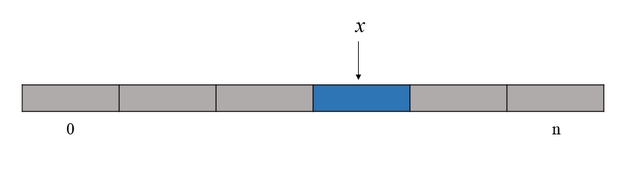
\includegraphics[width=0.9\textwidth]{Fig/array_1.png}
\caption{\footnotesize{Storing value \emph{x} in an array.}}
\label{fig:array}
\end{figure}
% ============================================================================== %

In order to look up the value \emph{x}, we have to iterate over the entire array as we do not know where is the exact place it is stored. This can be neglected in case of arrays with small size, however, it takes a long time to find an item as the array size grows.
On the other hand, in order to store the value \emph{x} in a mapping, user needs to provide a pair of (key, \emph{x}), then the key gets hashed and outputs a number which indicates where in the mapping \emph{x} should be stored (see Figure~\ref{fig:mapping}).
% ===============Mapping figure================================== %
\begin{figure}[htb!p]
\centering
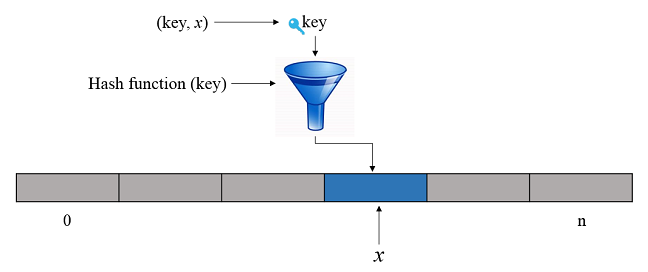
\includegraphics[width=0.9\textwidth]{Fig/mappingFig_2.png}
\caption{\footnotesize{Storing value \emph{x} in a mapping.}\label{tab:store}}
\label{fig:mapping}
\end{figure}
% ============================================================================== %
In order to retrieve the value \emph{x} from a mapping, user needs to provide the associated key, the key gets hashed and supplies the exact location where \emph{x} is stored in mapping. Note that hash functions are deterministic and they always generate the same hash value for a given input. Therefore, instead of iterating over the entire mapping, one only needs to provide the exact pair of (key, value) every time he wants to look up that value. 

According to what have been presented, mappings enjoy a higher level of efficiency in compared with arrays. Retrieving a value from array requires a full scan of the array which results in O(n) complexity, whereas with mapping, Searching for a value is performed in O(1) as it takes a constant time to find that value. Table~\ref{tab:complexity} summarizes the average complexity of performing the three \emph{insert}, \emph{search}, and \emph{delete} functions on arrays and mappings data structures. 
% ===============Mapping vs Array table================================== %
\begin{table}[h!]
\renewcommand{\arraystretch}{2}
\centering
 \begin{tabular}{||c | c | c||} 
 \hline
 Function & Arrays & Mappings\\ [2.5ex] 
 \hline\hline
Insert & O(1) & O(1)  \\ \hline
Search & O(n) & O(1)  \\ \hline
 Delete & O(n) & O(1)  \\[1ex] 
 \hline
 \end{tabular}
\caption{\footnotesize{Summary of performance characteristics of arrays and mappings.}}
\label{tab:complexity}
\end{table}
% ============================================================================== %
In view of all that has been mentioned so far, we select mappings to design and implement our system.


% ===============Enums================================== %
\subsubsection*{Enums}

Enums enable smart contract developers to create user-defined types in Solidity. In \Ghazalstar, we use enums data types to implement state machines and encapsulate functions' behavior based on a given state. Code~\ref{code:enumDS} is an example of using enums in \Ghazalstar. As the code shows, we create a user-defined type called \emph{States} to (i) define every possible states for a domain name and (ii) maintain the states of all domain names that exist within our system.

\emph{States} contains six values including \emph{unregistered, registered, expired, TLS key entered, DNS has entered, and TLS key\_DNS hash entered}. Each of these values indicates a possible state that every domain names may go through. Interestingly, enums can be explicitly converted to/from the any integer types \eg States(1) represents the \emph{registered} state.

Once the new data type is defined (line 1, Code~\ref{code:enumDS}), we can declare variables of that type that contain possible stages we have specified. Line 14 of Code~\ref{code:enumDS} represents declaring a new variable called \emph{state} as a domain struct's property. Using the \emph{state} variable, we can maintain domain name's possible states which we will further explain how it leads us to design \Ghazalstar namespace properly.


% ===============Enums Code in Ghazal================================== %

\begin{lstlisting} [basicstyle=\scriptsize\ttfamily,caption={Defining a new data type called \emph{States} and declaring a new variable called \textit{state} of that type in \Ghazalstar smart contract.},label={code:enumDS},float]
enum <@\textcolor{cyan}{States}@>{
	  Unregistered,
	  Registered,
	  Expired,
	  TLSKeyEntered,   
	  DNSHashEntered,
	  TLSKey_And_DNSHashEntered}
struct Domain{
    bytes32 DomainName;
        address DomainOwner;
        uint RegistrationTime;
        bytes32[] TLSKeys; 
        bool isValue; 
        States state; 
        ZoneFileStruct ZoneFile;}
\end{lstlisting}
%=======================================================================%

% ===============Function================================== %
\subsection{Functions}

Solidity allows developers to define units of code called \emph{functions} in smart contracts and execute those code on EVM. Solidity functions are classified into two types of (i) transactional, also known as functions, and (ii) constant. Transactional functions, as the name implies, generate a transaction to the Ethereum blockchain and can modify the state of a contract, once they are invoked. In contrast, constant functions cannot update the state of the contracts and modify the blockchain. Alternatively, they can be called to return a value to the user who directly calls these function without consuming any amount of gas. Functions can be described with four distinctive visibility marks in Solidity. These include: 
\begin{itemize}
\item External: These functions are part of the contract definition, although they can not be called and invoked internally and can be merely called by external entities within the blockchain (contracts and/or accounts).
\item Public: These functions are default in Solidity and do not need to be determined. Public functions can be accessed and invoked both internally or by external entities within the blockchain (contracts and/or accounts).
\item Internal: These functions can merely be accessed and invoked by the contract in which they are defined and its inherited functions and internal libraries.
\item Private: These functions can be merely accessed and invoked by the current contract in which they are defined and not by its inherited functions, internal libraries, and external entities within the blockchain (contracts and/or accounts).
\end{itemize}
% ===============Function Modifiers================================== %
\subsection{Function Modifiers}

Function modifiers allow smart contract developers to easily modify the behavior of functions. In solidity, every function can belong to different modifiers, that is, multiple conditions need to be satisfied in order for the function to be executed. At the time of writing the thesis, \Ghazalstar smart contract contains 11 function modifiers which enforce different conditions, what follows is a description of the five example of these modifiers.
% ===============costs Modifier================================== %
\subsubsection*{\emph{Costs} Function Modifier}

As mentioned previously, users can register and/or renew domain names by paying an certain amount of ether as domain registration fee in \Ghazalstar. To enforce that, the two \emph{register} and \emph{renew} functions are followed by the \emph{costs} modifier which requires a certain amount of fee to be associated with these function calls. Therefore, a user can only invoke and execute these function if he pays the amount that is specified as the registration fee. Additionally, in order to receive ether, these functions are marked \emph{payable}. \emph{costs} modifier first checks the condition prior to executing the function (line 2, Code~\ref{code:CostModifier}) and control flow continues after the "\_" in the modifier (line 3, Code~\ref{code:CostModifier}).

% ===============costs Modifier code================================== %
\begin{lstlisting} [basicstyle=\scriptsize\ttfamily,caption={Implementation of the \emph{Costs} modifier in \Ghazalstar smart contract.},label={code:CostModifier},float]
modifier Costs() {
        require(msg.value >= Registration_Fee); 
        _;   
    }
\end{lstlisting}
% ========================================================= %
\subsubsection*{\emph{OnlyOwner} Function Modifier}

In \Ghazalstar smart contract, we define the \emph{OnlyOwner} function modifier in a way that it requires a function to be only called from a certain Ethereum address. In fact, any time that a user calls a function on an specific domain name (\eg add TLS key), the \emph{OnlyOwner} modifier receives the domain name as its argument and allows the user to successfully execute the function only if he is the owner of that domain (see Code~\ref{code:OnlyOwner}). 

% ===============OnlyOwner Modifier code================================== %
\begin{lstlisting}[basicstyle=\scriptsize\ttfamily,caption={Implementation of the \emph{OnlyOwner} modifier in \Ghazalstar smart contract.},label={code:OnlyOwner},float]
modifier OnlyOwner(bytes32 _DomainName) {
        require (Domains[_DomainName].DomainOwner == msg.sender);
        _;
    }
\end{lstlisting}
% ========================================================= %
\subsubsection*{\emph{AtStage} and \emph{Not\_AtStage} Function Modifiers}

In Solidity, functions are atomic operations, that is to say, they can be invoked and executed at any time and any order irrespective of the actual order they are written in the smart contract. Therefore, in order to design interactions within the \Ghazalstar smart contract accurately, we use \emph{AtStage} and \emph{Not\_AtStage} function modifiers to model the states of the contract and prevent incorrect function calls by ensuring that functions can only be executed at certain stages (see Code~\ref{code:Stages}). For instance, using the \emph{AtStage} modifier, we enforce the \emph{register($D_i$)} function to be executed only if the $D_i$ is at \emph{unregistered} or \emph{expired} state.
% ===============AtStage and Not_AtStage Modifier code================================== %

\begin{lstlisting} [basicstyle=\scriptsize\ttfamily,caption={Implementation of the \emph{AtStage} and \emph{Not\_AtStage} function modifiers in \Ghazalstar smart contract.},label={code:Stages},float]
modifier AtStage(bytes32 _DomainName,States stage_1,States stage_2) {
        require (Domains[_DomainName].state == stage_1 ||     Domains[_DomainName].state == stage_2);
        _;
    }
    modifier Not_AtStage(bytes32 _DomainName,States stage_1,States stage_2) { 
        require (Domains[_DomainName].state != stage_1 ||     Domains[_DomainName].state != stage_2);
        _;
    }
\end{lstlisting}
%=========================================================%
\subsubsection*{\textit{CheckDomainExpiry} Function Modifier}

The \emph{CheckDomainExpiry} function modifier, as the name implies, applies the domains registration expiration after a certain period of time. This function modifier receives a domain name as its argument and changes its state to \emph{expired} if it meets the condition that is specified within the modifier's body (see Code~\ref{code:CheckDomainExpiry}, line 2)
% ===============CheckDomainExpiry Modifier code================================== %

\begin{lstlisting}[basicstyle=\scriptsize\ttfamily,caption={Implementation of the \emph{CheckDomainExpiry} function modifier in \Ghazalstar smart contract.},label={code:CheckDomainExpiry},float]
modifier CheckDomainExpiry (bytes32 _DomainName) {
        require (now >= Domains[_DomainName].RegistrationTime + 5 years);
        var DomainVar = Domains[_DomainName];
        DomainVar.state = States.Expired;
        Domains[_DomainName] = DomainVar;
        _;
    }
\end{lstlisting}
%=========================================================%
%==================Evaluation============================%
\section{Evaluation}
\label{sec:Evaluation}
So far this chapter has focused the Ethereum concepts and data structures in addition to \Ghazalstar smart contract's design and description of its components. The aim of Section~\ref{sec:Evaluation} is to provide the technical implementation details of our system on the Ethereum blockchain. We specifically discuss the costs related to the deployment of \Ghazalstar smart contract on the Ethereum blockchain in addition to executing its functions on the Ethereum virtual machine. Moreover, a smart contract analysis tool is used to analyze the security of our system against a several number of security threats to which smart contracts are often vulnerable.


%==================Deployment============================%
\subsection{Deployment}

In order to analyze the \Ghazalstar smart contract in today's Ethereum blockchain, Ropsten, Ethereum test network, has been used~\cite{GitHubet61:online}. Test networks replicate the Ethereum network and EVM as well as offering an inexpensive way for smart contract developers to test their codes. Ropsten is a public test network that entirely stimulates the Ethereum peer to peer network except that it provides free gas. Therefore, we successfully tested \Ghazalstar smart contract on this test network without paying the real cost of gas for our executions.
%==================Gas Estimation============================%
\subsection{Gas Estimation}

\Ghazal smart contract is implemented in 370 lines of Solidity language, a high level programming language resembles to JavaScript, and tested on the Ethereum test network. We use the Solidity compiler to evaluate the rough cost for publishing the \Ghazalstar smart contract on the Ethereum blockchain as well as the cost for the various operations to be executed on the Ethereum virtual machine. As of January 2018, 1 gas =  $21\times10^{-9}$ ether\footnote{https://ethstats.net/}, and 1 ether = \$882.92\footnote{https://coinmarketcap.com/}.

Table~\ref{tab:performance} represents the estimated costs for \Ghazalstar (and its inherited \Ghazal functionality) smart contract deployment and function invocation in both gas and USD. As it can be seen from both Table 1, the most considerable cost is the one-time cost paid to deploy the system on Ethereum. There are then relatively small costs associated with executing the functions, \ie users could easily register a domain by paying \$3.15 or they could bind a key to the domain they own for a cost of \$1.43, which is relatively cheap when compared with the real world costs associated with these operations.

%============= Ghazal with Auction Costs Table==================== %
\begin{table}[t]
\centering
\begin{tabular}{|l|l|l|l|}
\hline
\textbf{Operation} & \textbf{Gas} & \textbf{Gas Cost in Ether}  & \textbf{Gas Cost in USD}  \\ \hline
Register & 169 990 & $3.56\times10^{-3}$ & \$3.15\\
Renew & 54 545 & $1.14\times10^{-3}$ & \$1.01 \\
Transfer\textunderscore Domain & 53 160 & $1.11\times10^{-3}$ & \$0.98\\
Add\textunderscore TLSKey & 77 625 & $1.63\times10^{-3}$ & \$1.43 \\ 
Add\textunderscore ZoneFile & 57 141 &  $1.19\times10^{-3}$ & \$1.05 \\
Add\textunderscore TLSKey\textunderscore AND\textunderscore ZoneFile & 68 196 & $1.43\times10^{-3}$ & \$1.26\\
Revoke\textunderscore TLSkey & 37 672 & $7.91\times10^{-4}$ & \$0.69\\
StartAuction & 119 310 & $2.50\times10^{-3}$ & \$2.21\\
Bid & 112 491 & $2.36\times10^{-3}$ & \$2.08\\
Withdraw\textunderscore bids & 46 307 & $9.72\times10^{-4}$ & \$0.85\\
Withdraw\textunderscore deposits & 47 037 & $9.87\times10^{-4}$ & \$0.87\\
Settle & 77 709 & $1.63\times10^{-3}$ & \$1.44\\
\hline
\textbf{\Ghazalstar Contract Creation} & 2 402 563 & 0.05 & \$44.54\\
\hline
\end{tabular}
\caption{\footnotesize{Gas used for operations in the \Ghazalstar smart contract.}\label{tab:performance}}
\end{table}
%======================================== %
%=============Security Analysis==================== %
%======================================== %
\subsection{Security Analysis}

Ethereum smart contracts, in particular the ones implemented in Solidity, are notorious for programming pitfalls. As they generally transfer and handle assets of considerable value, bugs in Solidity code could result in serious vulnerabilities which can be exploited by adversaries. We use standard defensive programming approaches, in particular around functions that transfer money (such as the auction function that refunds the security deposits), by using explicitly coded state machines and locks, and by not making state-changes after transfers. We also analyze \Ghazalstar against Oyente, a symbolic execution tool proposed by Luu \etal\cite{luu2016making} which looks for potential security bugs like the re-entry attack (infamously). The results of the security analysis represent that both of the smart contracts are not vulnerable to any known critical security issue (see Figure~\ref{fig:oyente}).

%==============Oyente=================== %
\begin{figure}[t]
\centering
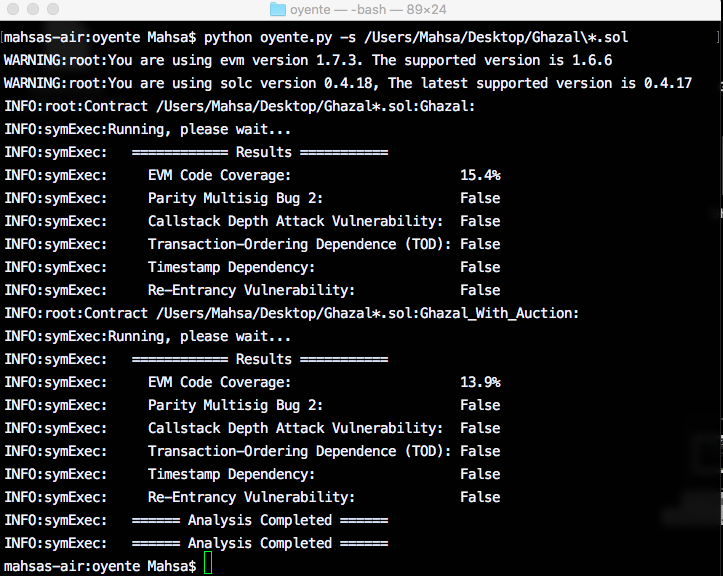
\includegraphics[width=0.8\textwidth]{Fig/GhazalstarOyenteResult.png}
\caption{\footnotesize{Results of \Ghazalstar security analysis using Oyente \cite{luu2016making}.}\label{fig:oyente}}
\end{figure}
%==================================== %

\section{Conclusion}

In this chapter, we described and discussed the main concepts of the Ethereum blockchain as well as the Solidity language. We also provided a few code snippets of \Ghazalstar to show a better understanding of our system. In the last section, a thorough security and cost evaluation of \Ghazalstar was performed. According to the results, our system is totally secure against the existing security vulnerabilities. The overall system costs under \$100 to deploy Basic actions like domain registration costs under \$5.


 